\documentclass[12pt]{extarticle} 
\usepackage{amsmath,amsfonts,amssymb,amsthm,graphicx,xcolor,natbib,booktabs,tabularx}
%\usepackage[paperwidth=126mm, paperheight=96mm, top=5mm, bottom=5mm, right=5mm, left=5mm]{geometry}
\usepackage[margin=1cm,footskip=5mm]{geometry}
\pagenumbering{gobble}

\usepackage[inline]{enumitem}
%\usepackage{unicode-math}
\usepackage[BoldFont,SlantFont]{xeCJK}  
\xeCJKsetemboldenfactor{2}
\setCJKmainfont{cwTeX Q Yuan Medium}
%\setCJKmainfont{cwTeX Q Kai Medium}
%\setCJKmainfont{cwTeX Q Ming Medium}
%\setCJKmainfont[AutoFakeSlant=.1,AutoFakeBold=1]{cwTeX Q Kai Medium} 
%\setCJKfamilyfont{kaiv}[Vertical=RotatedGlyphs]{cwTeX Q Medium}
%\setmainfont{texgyrepagella-regular.otf}
%\setmathfont{texgyrepagella-math.otf}
\usepackage{lmodern}
\newcommand{\ds}{\displaystyle}
\newcommand{\ie}{\;\Longrightarrow\;}
\newcommand{\ifff}{\;\Longleftrightarrow\;}
\newcommand{\mi}{\mathrm{i}}
\DeclareMathOperator*{\dom}{dom}
\DeclareMathOperator*{\codom}{codom}
\DeclareMathOperator*{\ran}{ran}
\newcommand{\floor}[1]{\lfloor #1 \rfloor}
\newcommand{\ceil}[1]{\lceil #1 \rceil}

\newcommand{\bdiff}[2]{ \frac{\mathrm{d}}{\mathrm{d}#2} \left( #1 \right)}
\newcommand{\ddiff}[3]{ \frac{\mathrm{d}^#1#2}{\mathrm{d}{#3}^#1}}
\newcommand{\half}{\tfrac{1}{2}}
\newcommand{\diff}[2]{ \frac{\mathrm{d}\hfil#1\hfil}{\mathrm{d}#2}}
\newcommand{\difftwo}[2]{ \frac{\mathrm{d^2}\hfil#1\hfil}{\mathrm{d}{#2}^2}}

% figure --> 圖
\renewcommand{\appendixname}{附錄}
\renewcommand{\figurename}{圖}
\renewcommand{\tablename}{表}
\renewcommand{\refname}{參考文獻}

\usepackage{hyperref}
\hypersetup{
    colorlinks,
    linkcolor={red!50!black},
    citecolor={blue!60!black},
    urlcolor={blue!60!black}
    %urlcolor={blue!80!black}
}

\theoremstyle{definition}
\newtheorem*{dfn}{定義}
\newtheorem*{prp}{性質}
\newtheorem*{fact}{結論}
\newtheorem*{thm}{定理}
\newtheorem*{ex}{例}
\newtheorem*{sol}{解}
\newtheorem*{prf}{證}
\newtheorem*{rmk}{註}

%\setenumerate{label=(\roman*),itemsep=1pt,topsep=3pt}
\newcommand{\myline}{\noindent\makebox[\linewidth]{\rule{\paperwidth}{0.4pt}}}
%\newcommand{\myline}{\textcolor[RGB]{220,220,220}{\rule{\linewidth}{1pt}}}

\usepackage{pgfplots}
\usetikzlibrary{arrows.meta,angles,quotes,patterns}
% axis style, ticks, etc
\pgfplotsset{every axis/.append style={
                   label style={font=\fontsize{4}{4}\selectfont},
                   tick label style={font=\fontsize{4}{4}\selectfont}  
               },
            }
\renewcommand\tabularxcolumn[1]{m{#1}}

%%%%%%%%%%%%%%%%%%%%%%%%%%%%%%%%%%%%%%%%%%%%%%%%%%%%%%%%%%%%%%%%%%%%%

\usepackage{multicol}
\usepackage{ifthen}
\tikzstyle{vertex}=[shape=circle, minimum size=2mm, inner sep=0, fill]
\tikzstyle{opendot}=[shape=circle, minimum size=2mm, inner sep=0, fill=white, draw]
\newcommand{\myaxis}[7][help lines]{%[formatting of lines]{xlabel}{xleft}{xright}{ylabel}{yleft}{yright}
	\ifthenelse{\lengthtest{#3 pt=0 pt}}{}{
		\draw[ <-,#1] (-#3,0)--(0,0);
		}
	\ifthenelse{\lengthtest{#4 pt=0 pt}}{
		\draw[#1] (0,0)node[right]{$#2$};}{
		\draw[ ->,#1] (0,0)--(#4,0)node[right]{$#2$};
		}
	\ifthenelse{\lengthtest{#6 pt= 0 pt}}{
		}{
		\draw[ <-,#1] (0,-#6)--(0,0);}
	\ifthenelse{\lengthtest{#7 pt= 0 pt}}{
		\draw[#1] (0,0)node[above]{$#5$};
		}{
		\draw[ ->,#1] (0,0)--(0,#7)node[above]{$#5$};}
}

% colorblind-friendly palette
% mixed colours: CB sees contrasting grays
\definecolor{M1}{RGB}{0,0,0}
\definecolor{M2}{RGB}{0,73,73}
\definecolor{M3}{RGB}{0,146,146}
\definecolor{M4}{RGB}{255,109,182}
\definecolor{M5}{RGB}{255,182,119}
% cool colours: CB sees contrasting blues
\definecolor{C1}{RGB}{73,0,146}
\definecolor{C2}{RGB}{0,109,219}
\definecolor{C3}{RGB}{182,109,255}
\definecolor{C4}{RGB}{109,182,255}
\definecolor{C5}{RGB}{182,219,255}
% warm colours: CB sees contrasting yellow
\definecolor{W1}{RGB}{146,0,0}
\definecolor{W2}{RGB}{146,73,0}
\definecolor{W3}{RGB}{219,209,0}
\definecolor{W4}{RGB}{36,255,36}
\definecolor{W5}{RGB}{255,255,109}

%%%%%%%%%%%%%%%%%%%%%%%%%%%%%%%%%%%%%%%%%%%%%%%%%%%%%%%%%%%%%%%%%%%%%

\usepackage{fancyhdr}
\fancypagestyle{firststyle} {
   \fancyhf{}
   \fancyfoot[R]{\footnotesize \DTMnow}
   \renewcommand{\headrulewidth}{0pt} 
}
\usepackage{datetime2}

\begin{document}
\title{\texorpdfstring{\vspace{-16mm} 第三章\ \ 微分應用}{第三章\ \ 微分應用}} 
\author{\vspace{-5em}}
\date{\vspace{-5em}}
\maketitle
\thispagestyle{firststyle}

\section*{3.1 均值定理}

\begin{thm}[Rolle]
  若 $f(x)$ 在 $[a, b]$ 連續, 在 $(a, b)$ 可微, 且 $f(a) = f(b)$, 則存在 $\ds c\in (a, b)$ 使 $\ds f'(c)=0$. 
\end{thm}
\vspace{-7mm}
\begin{figure}[!htbp]
  \centering
  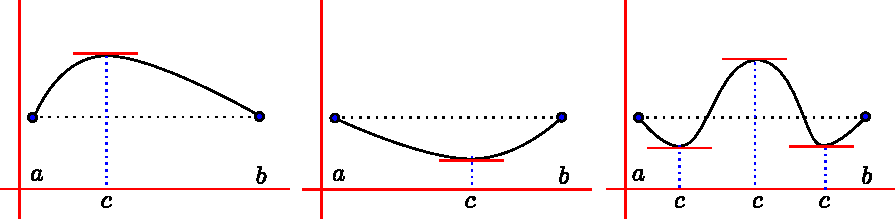
\includegraphics[scale=1,page=1]{fig/rolle.pdf}
\end{figure}

\begin{thm}[均值定理 (mean-value theorem, MVT) ]
  若 $f(x)$ 在 $[a, b]$ 連續, 在 $(a, b)$ 可微, 則存在 $\ds c\in (a, b)$ 使 $\ds f'(c) = \frac{f(b) - f(a)}{b - a}$. 
\end{thm}
\vspace{-1cm}
\begin{figure}[!htbp]
  \centering
  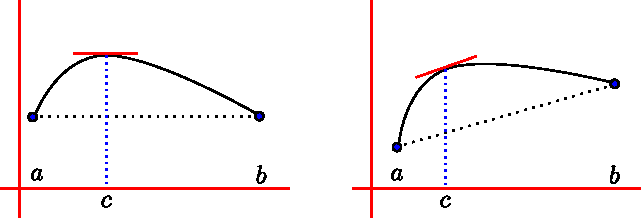
\includegraphics[scale=1,page=1]{fig/rolle_to_mvt.pdf}
\end{figure}

\begin{rmk} 不滿足『$f(x)$ 在 $[a, b]$ 連續, 在 $(a, b)$ 可微』時的反例.  
  \begin{itemize}\setlength\itemsep{0em}
    \item 令 $a=0$, $b=2$, 且 
    \smallskip
    \begin{align*}
      f(x) = \begin{cases} 0 & \text{若 }\; x \leqslant 1 \\ 1 & \text{若 }\; x > 1\end{cases}
      \hskip0.8in  \smash{\raisebox{-0.5\height}{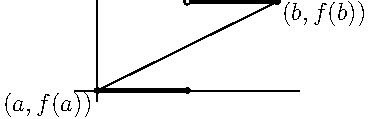
\includegraphics{fig/mvtd.pdf}}}
    \end{align*}
    \medskip
    \noindent
    當 $x\ne 1$ 時 $f'(x) = 0$, 但連接 $\ds(a,\,f(a))=(0,\,0)$ 與 $\ds(b,\,f(b))=(2,\,1)$ 之割線斜率為 $\ds\frac{1}{2}$. 
   \item 令 $a=-1$, $b=1$, $f(x)=|x|$. 
    \smallskip
    \begin{align*}
      f'(x) = \begin{cases} -1  & \text{若 }\;x < 0 \\ \text{DNE} & \text{若 }\; x = 0\\ 1 & \text{若 }\; x > 0\end{cases}
      \hskip0.8in  \smash{\raisebox{-0.5\height}{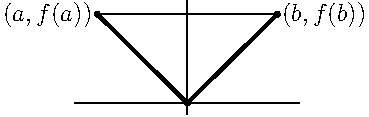
\includegraphics{fig/mvte.pdf}}}
    \end{align*}
    \smallskip
    \noindent
    當 $x\ne 0$ 時 $f'(x)=\pm 1$, 但連接 $(a,\,f(a))=(-1,\,1)$ 與 $(b,\,f(b))=(1,\,1)$ 之割線斜率為 $0$. 
  \end{itemize}
\end{rmk}

\begin{prp}
  $f(x)$ 在 $[a, b]$ 連續, 在 $(a, b)$ 可微. 若 $\ds\forall\,x\in(a, b)$ 
  \begin{multicols}{2}
    \begin{enumerate}\setlength\itemsep{0em}
      \item $f'(x) > 0$ $\ifff$ $f$ 在 $[a, b]$ 嚴格遞增. 
      \item $f'(x) < 0$ $\ifff$ $f$ 在 $[a, b]$ 嚴格遞減. 
      \item $f'(x) \geqslant 0$ $\ifff$ $f$ 在 $[a, b]$ 遞增. 
      \item $f'(x) \leqslant 0$ $\ifff$ $f$ 在 $[a, b]$ 遞減. 
    \end{enumerate}
  \end{multicols}
\end{prp}

\begin{prf}
  令 $\ds x$, $y\in[a, b]$, $x < y$. 由 MVT $\ds\exists\,c\in(x, y)\subseteq(a, b)$ 使 $\ds f(y) - f(x) = f'(c)\,(y - x)$. 又 $y - x > 0$, $f(y) - f(x)$ 與 $f'(c)$ 同號.  
\end{prf}

\begin{fact}
  若 $f(x)$, $g(x)$ 在 $[a, b]$ 連續, 在 $(a, b)$ 可微, 且 $f'(x) = g'(x)\;\forall\,x\in(a, b)$, 則存在 $C\in\mathbb{R}$ 使 $f(x) = g(x) + C,\;\forall\,x\in[a, b]$. 
\end{fact}

\begin{ex}
  證明 $\ds 2x - 1 = \sin x$ 僅有唯一解. 
\end{ex}

\begin{sol}
  令 $\ds f(x) = 2 x - 1 - \sin x$, 則 $\ds\forall\,x\;(f'(x) = 2 - \cos x > 0)$, $f(0) = -1 < 0$, $f(1) = 1 - \sin 1 > 0$, 故由 Bolzano 定理, 存在 $\ds c\in(0, 1)$ 使 $f(c) = 0$. 若存在另一 $c_0\ne c$ 使 $f(c_0) = 0$, 則由 Rolle 定理, 存在 $c_1$ 介於 $c$, $c_0$ 間使 $f'(c_1) = 0$, 與 $\ds\forall\,x\;(f'(x) = 2 - \cos x > 0)$ 矛盾; 得證. 
\end{sol}

\begin{ex}
  證明 $\ds x^3 + e^x = 0$ 僅有唯一解. 
\end{ex}

\begin{sol}
  令 $\ds f(x) = x^3 + e^x$, 則 $\ds\forall\,x\;(f'(x) = 3 x^2 + e^x > 0)$, $f(-1) = -1 + e^{-1} < 0$, $f(0) = 1 > 0$, 故由 Bolzano 定理, 存在 $\ds c\in(-1, 0)$ 使 $f(c) = 0$. 若存在另一 $c_0\ne c$ 使 $f(c_0) = 0$, 則由 Rolle 定理, 存在 $c_1$ 介於 $c$, $c_0$ 間使 $f'(c_1) = 0$, 與 $\ds\forall\,x\;(f'(x) = 3 x^2 + e^x > 0)$ 矛盾; 得證. 
\end{sol}

\begin{ex}
  證明 $\ds\ln\big(1 + \frac{1}{x}\big) > \frac{1}{1 + x}$, $\forall\,x > 0$. 
\end{ex}

\begin{sol}
  考慮 $\ds\ln t$ 在 $\ds[x, x + 1]$, $\ds x > 0$. 由 MVT $\ds\exists\,c\in(x, x + 1)\;\ln(x + 1) - \ln x = \frac{1}{c} > \frac{1}{x + 1}$. 
\end{sol}

\begin{ex}
  證明 $\ds\tan x > x$, $\ds\forall\,x\in\big(0, \frac{\pi}{2}\big)$. 
\end{ex}

\begin{sol}
  $\ds\forall\,x\in\big(0, \frac{\pi}{2}\big)$, $\ds\tan$ 在 $[0, x]$ 連續, 在 $(0, x)$ 可微, 故由 MVT $\ds\exists\,c\in(0, x)\;\tan x - \tan 0 = \sec^2 c\cdot x > x$. 
\end{sol}

\begin{ex}
  證明 $\ds\frac{2}{\pi} < \frac{\sin x}{x} < 1$, $\ds\forall\,x\in\big(0, \frac{\pi}{2}\big)$. 
\end{ex}

\begin{sol}
  令 $\ds g(x) = \begin{cases}\frac{\sin x}{x} & \text{若}\;x\ne 0 \\ 1 & \text{若}\;x = 0 \end{cases}$, 則 $g$ 為連續, 且 $\ds\forall\,x\in\Big(0,\frac{\pi}{2}\Big)\quad g'(x) = \frac{x\cos x - \sin x}{x^2} = \frac{\cos x}{x^2}(x - \tan x) < 0$ $\ie$ $g$ 在 $\ds\Big(0,\frac{\pi}{2}\Big)$ 為嚴格遞減函數 $\ie$ $\ds\frac{2}{\pi} = g\,\Big(\frac{\pi}{2}\Big) < g(x) = \frac{\sin x}{x} < g(0) = 1$     
\end{sol}

\begin{ex}
  證明 $\ds\sqrt{1 + x} < 1 + \frac{1}{2}x$, $\forall\,x > 0$. 
\end{ex}

\begin{sol}
  考慮 $\ds\sqrt{1 + t}$ 在 $\ds[0, x]$, $\ds x > 0$. 由 MVT $\ds\exists\,c\in(0, x)\;\sqrt{1 + x} - \sqrt{1} = \frac{1}{2\sqrt{1 + c}} x < \frac{1}{2}x \ie \sqrt{1 + x} < 1 + \frac{1}{2}x$. 
\end{sol}

\begin{ex}
  證明 $\ds\sin^{-1}x + \cos^{-1}x = \frac{\pi}{2}$, $\forall\,x\in[-1, 1]$. 
\end{ex}

\begin{sol}
  令 $\ds f(x) = \sin^{-1}x + \cos^{-1}x$. $\forall\,x\in(-1, 1)$, $\ds f'(x) = \frac{1}{\sqrt{1 - x^2}} + \frac{-1}{\sqrt{1 - x^2}} = 0$ $\ie$ $f(x)$ 為常數 $\ie$ $\ds f(x) = f(0) = \frac{\pi}{2}$; 由 $f(x)$ 之連續性或代入 $x = \pm 1$ 均可得 $\ds f(\pm 1) = \frac{\pi}{2}$.    
\end{sol}

\begin{ex}
  證明 $\ds 2\sin^{-1}x = \cos^{-1}(1 - 2x^2)$, $\forall\,x\in[0, 1]$. 
\end{ex}

\begin{sol}
  令 $\ds f(x) = 2\sin^{-1}x - \cos^{-1}(1 - 2x^2)$. $\forall\,x\in(0, 1)$, $\ds f'(x) = \frac{2}{\sqrt{1 - x^2}} - \frac{4x}{\sqrt{1 - (1 - 2x^2)^2}} = \frac{2}{\sqrt{1 - x^2}} - \frac{4x}{\sqrt{(2 - 2x^2)2x^2}} = \frac{2}{\sqrt{1 - x^2}} - \frac{4x}{2x\sqrt{(1 - x^2)}} = 0$ $\ie$ $f(x)$ 為常數 $\ie$ $\ds f(x) = f\Big(\frac{1}{2}\Big) = 2\cdot\frac{\pi}{6} - \frac{\pi}{3} = 0$; 由 $f(x)$ 之連續性或代入 $x = 0$, $1$ 均可得 $f(0) = 0 = f(1)$.   
\end{sol}

\begin{ex}
  證明 $\ds\sin^{-1}\frac{x - 1}{x + 1} = 2\,\tan^{-1}\sqrt{x} - \frac{\pi}{2}$, $\forall\,x\geqslant 0$. 
\end{ex}

\begin{sol}
  令 $\ds f(x) = \sin^{-1}\frac{x - 1}{x + 1} - 2\,\tan^{-1}\sqrt{x} + \frac{\pi}{2}$. $\forall\,x > 0$, $\ds f'(x) = \frac{1}{\sqrt{1 - (\frac{x - 1}{x + 1})^2}}\cdot\frac{(x + 1) - (x - 1)}{(x + 1)^2} - 2\,\frac{1}{(\sqrt{x})^2 + 1}\cdot\frac{1}{2\sqrt{x}} = \frac{1}{\sqrt{\frac{(x + 1)^2 - (x - 1)^2}{(x + 1)^2}}}\cdot\frac{2}{(x + 1)^2} - \frac{1}{(x + 1)\sqrt{x}} = \frac{1}{\sqrt{x}\sqrt{(x + 1)^2}} - \frac{1}{(x + 1)\sqrt{x}} = \frac{1}{\sqrt{x}|x + 1|} - \frac{1}{(x + 1)\sqrt{x}} = 0$ $\ie$ $f(x)$ 為常數 $\ie$ $\ds f(x) = f(1) = -2\cdot\frac{\pi}{4} + \frac{\pi}{2} = 0$; 由 $f(x)$ 之連續性或代入 $x = 0$ 均可得 $f(0) = 0$.   
\end{sol}

\section*{3.2 L'H\^opital 法則}

%\begin{thm}
%  \begin{itemize}
%    \item[]
%    \item $\big(\frac{0}{0}\text{ 型}\big)$
%      \begin{itemize}
%        \item $\exists\,\delta > 0$ s.t. $\forall\,x\in(a, a + \delta)$, $f(x)$, $g(x)$ 可微且 $g(x)\ne 0$. 
%        \item $\ds\lim_{x\to a+}f(x) = \lim_{x\to a+}g(x) = 0$. 
%        \item $\ds\lim_{x\to a+}\frac{f'(x)}{g'(x)} = l\in\overline{\mathbb{R}}$. 
%      \end{itemize}
%    則 $\ds\lim_{x\to a+}\frac{f(x)}{g(x)} = l$. 
%    \item $\big(\frac{\infty}{\infty}\text{ 型}\big)$ 
%      \begin{itemize}
%        \item $\exists\,\delta > 0$ s.t. $\forall\,x\in(a, a + \delta)$, $f(x)$, $g(x)$ 可微. 
%        \item $\ds\lim_{x\to a+}|f(x)| = \lim_{x\to a+}|g(x)| = \infty$. 
%        \item $\ds\lim_{x\to a+}\frac{f'(x)}{g'(x)} = l\in\overline{\mathbb{R}}$. 
%      \end{itemize}
%    則 $\ds\lim_{x\to a+}\frac{f(x)}{g(x)} = l$. 
%    \item  (適當修改後) 上述 $a+$ 可以是 $a-$, $a$; $a$ 可以是 $\pm\infty$. 
%  \end{itemize}
%\end{thm}

\begin{thm}[L'H\^opital 法則 (LHR) ]
  若 $f$ 與 $g$ 為實可微函數, 且在 $(a, b)$ 上 $g'(x)\ne 0$ ($a,\,b\in\overline{\mathbb{R}}$) . 假設 
  \begin{align*}
    \lim_{x\to a+}f(x) = \lim_{x\to a+}g(x) = 0\quad\Big(\frac{0}{0}\;\text{型}\Big)\qquad\text{或}\qquad\lim_{x\to a+}g(x) = \infty\quad\Big(\frac{\infty}{\infty}\;\text{型}\Big)
  \end{align*}
  若 $\ds\lim_{x\to a+}\frac{f'(x)}{g'(x)} = L\in\overline{\mathbb{R}}$, 則 $\ds\lim_{x\to a+}\frac{f(x)}{g(x)} = L$. 
\end{thm}

\begin{table}[!htbp]
  \centering
  \scalebox{1}{
  \begin{tabular}{cccccccc} 
    \toprule
    \addlinespace[2mm]
    不定型 & $\ds\frac{0}{0}$ & $\ds\frac{\infty}{\infty}$ & $\ds 0\cdot\infty$ & $\ds \infty - \infty$ & $\ds 0^0$ & $\ds \infty^0$ & $\ds 1^\infty$ \\
    \addlinespace[2mm]
    \midrule
    \addlinespace[2mm]
    範例 & $\ds\lim_{x\to\frac{\pi}{2}}\frac{1 - \sin x}{1 + \cos 2x}$ & $\ds\lim_{x\to\infty}\frac{x^2}{e^x}$ & $\ds\lim_{x\to 0+}x\ln\frac{1}{x}$ & $\ds\lim_{x\to 1+}\Big(\frac{x}{x - 1} - \frac{1}{\ln x}\Big)$ & $\ds\lim_{x\to 0+} x^x$ & $\ds\lim_{x\to\infty} x^{\frac{1}{x}}$ & $\ds\lim_{x\to\infty} \Big(1 + \frac{a}{x}\Big)^{bx}$ \\ 
    \addlinespace[2mm]
    \bottomrule  
  \end{tabular}}
\end{table}

\begin{ex}[$\frac{0}{0}$]
  求 $\ds\lim_{x\to\frac{\pi}{2}}\frac{1 - \sin x}{1 + \cos 2x}$.  
\end{ex}

\begin{sol}
  $\ds\lim_{x\to\frac{\pi}{2}}\frac{1 - \sin x}{1 + \cos 2x} = \lim_{x\to\frac{\pi}{2}}\frac{-\cos x}{-2\sin 2x} = \lim_{x\to\frac{\pi}{2}}\frac{-1}{-4\sin x} = \frac{1}{4}$. 
\end{sol}

\begin{ex}[$\frac{\infty}{\infty}$]
  求 $\ds\lim_{x\to\infty}\frac{x^2}{e^x}$. 
\end{ex}

\begin{sol}
  $\ds\lim_{x\to\infty}\frac{x^2}{e^x} = \lim_{x\to\infty}\frac{2 x}{e^x} = \lim_{x\to\infty}\frac{2}{e^x} = 0$. 
\end{sol}

\begin{ex}[$0\cdot\infty$]
  求 $\ds\lim_{x\to 0+}x\ln\frac{1}{x}$. 
\end{ex}

\begin{sol}
  $\ds\lim_{x\to 0+}x\ln\frac{1}{x} = \lim_{x\to 0+}\frac{\ln\frac{1}{x}}{\frac{1}{x}} = \lim_{x\to 0+}\frac{-\frac{1}{x}}{-\frac{1}{x^2}} = \lim_{x\to 0+} x = 0$. 
\end{sol}

\begin{ex}[$\infty - \infty$]
  求 $\ds\lim_{x\to 1+}\Big(\frac{x}{x - 1} - \frac{1}{\ln x}\Big)$. 
\end{ex}

\begin{sol}
  $\ds\lim_{x\to 1+}\Big(\frac{x}{x - 1} - \frac{1}{\ln x}\Big) = \lim_{x\to 1+}\frac{x\ln x - (x - 1)}{(x - 1)\ln x} = \lim_{x\to 1+}\frac{1 + \ln x - 1}{(x - 1)\frac{1}{x} + \ln x} = \lim_{x\to 1+}\frac{\frac{1}{x}}{\frac{1}{x^2} + \frac{1}{x}} = \frac{1}{2}$. 
\end{sol}

\begin{ex}[$0^0$]
  求 $\ds\lim_{x\to 0+} x^x$. 
\end{ex}

\begin{sol}
  求 $\ds\lim_{x\to 0+} x^x = \lim_{x\to 0+} \exp\{x\ln x\} = \exp\big\{\lim_{x\to 0+} x\ln x\big\} = \exp\Big\{-\lim_{x\to 0+} x\ln\frac{1}{x}\Big\} = e^0 = 1$. 
\end{sol}

%\begin{ex}[$\infty^0$]
%  求 $\ds\lim_{x\to \frac{\pi}{2}-} (\tan x)^{\cos x}$.  
%\end{ex}
%
%\begin{sol}
%  $\ds\lim_{x\to \frac{\pi}{2}-} (\tan x)^{\cos x} = \lim_{x\to \frac{\pi}{2}-} e^{\cos x\ln(\tan x)} = e^{\lim_{x\to \frac{\pi}{2}-}\cos x\ln(\tan x)} = e^{\lim_{x\to \frac{\pi}{2}-}\frac{\ln(\tan x)}{\sec x}} = e^{\lim_{x\to \frac{\pi}{2}-}\frac{\frac{1}{\tan x}\sec^2 x}{\sec x\tan x}} \\ = e^{\lim_{x\to \frac{\pi}{2}-}\frac{\sec x}{\tan^2 x}} = e^{\lim_{x\to \frac{\pi}{2}-}\frac{\sec x\tan x}{2\tan x\sec^2 x}} = e^{\lim_{x\to \frac{\pi}{2}-}\frac{1}{2\sec x}} = e^0 = 1$.  
%\end{sol}

\begin{ex}[$\infty^0$]
  求 $\ds\lim_{x\to\infty} x^{\frac{1}{x}}$.  
\end{ex}

\begin{sol}
  $\ds\lim_{x\to\infty} x^{\frac{1}{x}} = \lim_{x\to\infty}\exp\big\{\ln x^{\frac{1}{x}}\big\} = \lim_{x\to\infty}\exp\Big\{\frac{1}{x}\ln x\Big\} = \exp\Big\{\lim_{x\to\infty}\frac{\ln x}{x}\Big\} = \exp\Big\{\lim_{x\to\infty}\frac{\frac{1}{x}}{1}\Big\} = e^0 = 1$.  
\end{sol}

\begin{ex}[$1^\infty$]
  求 $\ds\lim_{x\to\infty} \Big(1 + \frac{a}{x}\Big)^{bx}$, $a,\;b\in\mathbb{R}$. 
\end{ex}

\begin{sol}
  $\ds\lim_{x\to\infty} \Big(1 + \frac{a}{x}\Big)^{bx} = \lim_{x\to\infty} \exp\Big\{\ln\big(1 + \frac{a}{x}\big)^{bx}\Big\} = \lim_{x\to\infty} \exp\Big\{bx\,\ln\big(1 + \frac{a}{x}\big)\Big\} = \exp\Big\{\lim_{x\to\infty} bx\,\ln\big(1 + \frac{a}{x}\big)\Big\} = \exp\bigg\{b\lim_{x\to\infty}\frac{\ln(1 + \frac{a}{x})}{\frac{1}{x}}\bigg\} = \exp\bigg\{b\lim_{x\to\infty}\frac{\frac{1}{1 + \frac{a}{x}}\cdot\frac{-a}{x^2}}{\frac{-1}{x^2}}\bigg\} = \exp\bigg\{b\lim_{x\to\infty}\frac{a}{1 + \frac{a}{x}}\bigg\} = e^{ba}$. 
\end{sol}

\begin{ex}[循環形]
  求 $\ds\lim_{x\to\infty}\frac{e^x + e^{-x}}{e^x - e^{-x}}$. 
\end{ex}

\begin{sol}
  $\ds\lim_{x\to\infty}\frac{e^x + e^{-x}}{e^x - e^{-x}}$ 為 $\frac{\infty}{\infty}$ 型, 理應可使用 LHR, 但 $\ds\lim_{x\to\infty}\frac{e^x + e^{-x}}{e^x - e^{-x}} = \ds\lim_{x\to\infty}\frac{e^x - e^{-x}}{e^x + e^{-x}} = \lim_{x\to\infty}\frac{e^x + e^{-x}}{e^x - e^{-x}} = \ldots$, 無限循環; $\ds\lim_{x\to\infty}\frac{e^x + e^{-x}}{e^x - e^{-x}} = \lim_{x\to\infty}\frac{e^x\,(1 + e^{-2x})}{e^x\,(1 - e^{-2x})} = \lim_{x\to\infty}\frac{1 + e^{-2x}}{1 - e^{-2x}} = 1$. 
\end{sol}

\begin{ex}[LHR 與 DNE]
  若 $\ds\lim_{x\to a}f(x) = 0$, $\ds\lim_{x\to a}g(x) = 0$ 與 $\ds\lim_{x\to a}\frac{f'(x)}{g'(x)} = \text{DNE}$, $\ds\lim_{x\to a}\frac{f(x)}{g(x)}$ 仍可能存在: 取 $\ds f(x) = x^2\sin\frac{1}{x}$, $g(x)= x$ 與 $a = 0$, 則 $\ds\lim_{x\to 0} f(x) = 0$ 且 $\ds\lim_{x\to 0} g(x) = 0$, $\ds\lim_{x\to 0}\frac{f'(x)}{g'(x)} = \lim_{x\to 0}\left(2x\sin\frac{1}{x} -\cos\frac{1}{x}\right) = \text{DNE}$, 但 $\ds\lim_{x\to 0}\frac{f(x)}{g(x)} = \lim_{x\to 0}\frac{x^2\sin\frac{1}{x}}{x} = \lim_{x\to 0} x\sin\frac{1}{x}= 0$. 
\end{ex}

\section*{3.3 極值問題}

\begin{dfn}
  給定 $f:I\to\mathbb{R}$, $\ds B(x, h)\equiv\{y\;|\;|y - x| < h\}$. 
  \begin{itemize}\setlength\itemsep{0em}
    \item $f$ 在 $\ds x_\text{M}\in I$ 有最大值 (global maximum) $\ds f(x_\text{M})$: $\ds f(x_\text{M})\geqslant f(x),\;\forall\,x\in I$. 
    \item $f$ 在 $\ds x_\text{m}\in I$ 有最小值 (global minimum) $\ds f(x_\text{m})$: $\ds f(x_\text{m})\leqslant f(x),\;\forall\,x\in I$. 
    \item $f$ 在 $\ds x_0\in I$ 有極大值 (local maximum) $\ds f(x_0)$: $\ds\exists\,h_0 > 0$ 使 $\ds f(x_0)\geqslant f(x),\;\forall\,x\in B(x_0, h_0)\,\cap\,I$. 
    \item $f$ 在 $\ds x_1\in I$ 有極小值 (local minimum) $\ds f(x_1)$: $\ds\exists\,h_1 > 0$ 使 $\ds f(x_1)\leqslant f(x),\;\forall\,x\in B(x_1, h_1)\,\cap\,I$. 
  \end{itemize}
\end{dfn}

\begin{figure}[!htbp]
  \centering
  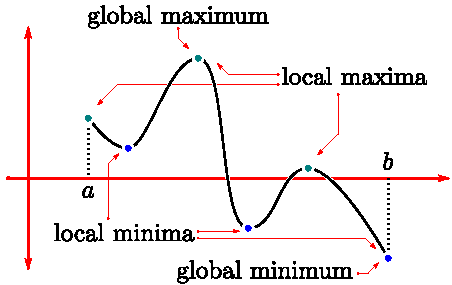
\includegraphics[scale=1,page=1]{fig/maxmin3.pdf}
  \hspace{25mm}
  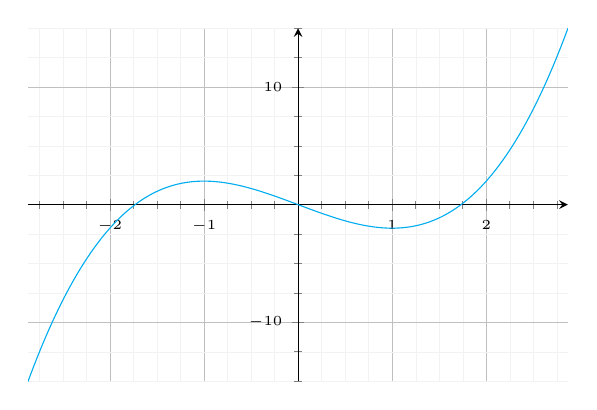
\begin{tikzpicture}[scale=1]
    \begin{axis}%
      [grid=both,
       unit vector ratio={8 1},
       minor tick num=3,
       ymin=-15,ymax=15,
       grid style={line width=.1pt, draw=gray!10},
       major grid style={line width=.2pt,draw=gray!50},
       axis lines=middle
      ]
      \addplot[domain=-3:3,samples=3000,smooth,cyan] {x^3 - 3 * x};
    \end{axis}
  \end{tikzpicture}
\end{figure}

\begin{ex}
  %\begin{multicols}{2}
  \begin{itemize}\setlength\itemsep{0em}
    \item[]
    \item $\ds f(x) = \sin x$ 在 $I = \mathbb{R}$ 有最大值 $1$, 最小值 $-1$. 
    \item $\ds f(x) = \frac{1}{x}$ 在 $I = \mathbb{R}$ 沒有最大值, 最小值. 
    \item $\ds f(x) = x$ 在 $I = (0, 1)$ 沒有最大值, 最小值. 
    \item $\ds f(x) = x$ 在 $I = [0, 1]$ 有最大值 $1$, 最小值 $0$. 
    \item 若 $I = [-3,\,3]$, $\ds f(x) = x^3 - 3x$ 在 $x = 3$ 有最大值 $18$, 在 $x = -3$ 有最小值 $-18$, 在 $x = -1$ 有極大值 $2$, 在 $x = 1$ 有極小值 $-2$. 
  \end{itemize}
  %\end{multicols}
\end{ex}

\begin{thm}
  若函數在定義域為{\color{M4}有限閉區間}, 或{\color{M4}有限閉區間的有限聯集}連續, 則函數在定義域上有最大值及最小值. 
\end{thm}

\begin{thm}
  若 $f(x)$ 在 $(a, b)$ 連續, 且 $\ds\lim_{x\to a+}f(x) = L$, $\ds\lim_{x\to b-}f(x) = M$. 
  \begin{enumerate}\setlength\itemsep{0em}
    \item 若 $\exists\,u\in(a, b)$ 使 $f(u) > L$ 且 $f(u) > M$, 則 $f$ 在 $(a, b)$ 有最大值. 
    \item 若 $\exists\,u\in(a, b)$ 使 $f(u) < L$ 且 $f(u) < M$, 則 $f$ 在 $(a, b)$ 有最小值. 
  \end{enumerate}
  $a$ 可為 $-\infty$, $b$ 可為 $\infty$, $L$, $M$ 可為 $\pm\infty$. 
\end{thm}

\begin{prf}
  \begin{enumerate}\setlength\itemsep{0em}
    \item[]
    \item 
    \begin{itemize}\setlength\itemsep{0em}
      \item 由 $\ds\lim_{x\to a+}f(x) = L$, 給定 $\varepsilon > 0$, $\exists\,\delta_1 > 0$ 使得當 $a < x < a + \delta_1$, $f(x) < L + \varepsilon$. 
      \item 取 $\varepsilon = f(u) - L$, 則
        \begin{align}\label{joi}
          \exists\,x_1\in (a, u) \text{ 使得當 }\; a < x < x_1, \,f(x) < L + (f(u) - L) = f(u).
        \end{align}
      \item 由 $\ds \lim_{x\to b-}f(x) = M$, 給定 $\varepsilon > 0$, $\exists\,\delta_2 > 0$ 使得當 $b - \delta_2 < x < b$, $f(x) < M + \varepsilon$. 
      \item 取 $\varepsilon = f(u) - M$, 則
        \begin{align}\label{jio}
          \exists\,x_2\in (u, b)\text{ 使得當 }\; x_2 < x < b, \,f(x) < M + (f(u) - M) = f(u).
        \end{align}
      \item 因 $f$ 在 $[x_1, x_2]$ 連續, $f$ 在 $w\in[x_1, x_2]$ 有最大值. 但 $u\in[x_1, x_2]\ie f(w)\geqslant f(u)$;  由 \eqref{joi}, \eqref{jio}, $f$ 在 $w\in(a, b)$ 有最大值. 
    \end{itemize}
  \item 
    \begin{itemize}\setlength\itemsep{0em}
      \item 由 $\ds \lim_{x\to a+}f(x) = L$, 給定 $\varepsilon > 0$, $\exists\,\delta_1 > 0$ 使得當 $a < x < a + \delta_1$, $f(x) > L - \varepsilon$. 
      \item 取 $\varepsilon = L - f(u)$, 則
        \begin{align}\label{joiw}
          \exists\,x_1\in (a, u) \text{ 使得當 }\; a < x < x_1, \,f(x) > L - (L - f(u)) = f(u).
        \end{align}
      \item 由 $\ds \lim_{x\to b-}f(x) = M$, 給定 $\varepsilon > 0$, $\exists\,\delta_2 > 0$ 使得當 $b - \delta_2 < x < b$, $f(x) > M - \varepsilon$. 
      \item 取 $\varepsilon = M - f(u)$, 則
        \begin{align}\label{jiow}
          \exists\,x_2\in (u, b)\text{ 使得當 }\; x_2 < x < b, \,f(x) > M - (M - f(u)) = f(u).
        \end{align}
      \item 因 $f$ 在 $[x_1, x_2]$ 連續, $f$ 在 $w\in[x_1, x_2]$ 有最小值. 但 $u\in[x_1, x_2]\ie f(w)\leqslant f(u)$;  由 \eqref{joiw}, \eqref{jiow}, $f$ 在 $w\in(a, b)$ 有最小值. 
    \end{itemize}
  \end{enumerate}
\end{prf}

\begin{thm}
  若 $f$ 在 $c\in\dom f$ 有極值, 且 $f'(c)$ 存在, 則 $f'(c) = 0$. 
\end{thm}

\begin{prf}
  \begin{itemize}\setlength\itemsep{0em}
    \item[]
    \item 若 $f$ 在 $c$ 有極大值, 則 $\ds\exists\,h_0 > 0$ 使 $\ds f(c)\geqslant f(x),\;\forall\,x\in B(c, h_0)\,\cap\,\dom{f}$. 
      \begin{itemize}\setlength\itemsep{0em}
      \item 取 $\ds x \in B(c, h_0)\,\cap\,\dom{f}$ 且 $x < c$, $\ds\frac{f(x) - f(c)}{x - c} \geqslant 0 \ie f'(c) = \lim_{x\to c-}\frac{f(x) - f(c)}{x - c}\geqslant 0$
      \item 取 $\ds x \in B(c, h_0)\,\cap\,\dom{f}$ 且 $x > c$, $\ds\frac{f(x) - f(c)}{x - c} \leqslant 0 \ie f'(c) = \lim_{x\to c+}\frac{f(x) - f(c)}{x - c}\leqslant 0$
    \end{itemize}
    故 $f'(c) = 0$. 
  \item 若 $f$ 在 $c$ 有極小值, 則 $\ds\exists\,h_1 > 0$ 使 $\ds f(c)\leqslant f(x),\;\forall\,x\in B(c, h_1)\,\cap\,\dom{f}$. 
    \begin{itemize}\setlength\itemsep{0em}
      \item 取 $\ds x \in B(c, h_1)\,\cap\,\dom{f}$ 且 $x < c$, $\ds\frac{f(x) - f(c)}{x - c} \leqslant 0 \ie f'(c) = \lim_{x\to c-}\frac{f(x) - f(c)}{x - c}\leqslant 0$
      \item 取 $\ds x \in B(c, h_1)\,\cap\,\dom{f}$ 且 $x > c$, $\ds\frac{f(x) - f(c)}{x - c} \geqslant 0 \ie f'(c) = \lim_{x\to c+}\frac{f(x) - f(c)}{x - c}\geqslant 0$
    \end{itemize}
    故 $f'(c) = 0$. 
  \end{itemize}
\end{prf}

\begin{fact}
  設 $f:I\to\mathbb{R}$ 在 $x_0\in I$ 有極值, 則 $x_0$ 為以下三情形之一: 
  \begin{multicols}{2}
    \begin{itemize}\setlength\itemsep{0em}
      \item 臨界點 (critical point) : $\ds f'(x_0) = 0$. 
      \item 奇異點 (singular point) : $f$ 在 $x_0$ 不可微.  
      \item $I$ 的邊界點 (boundary). 
    \end{itemize}
  \end{multicols}
\end{fact}

\begin{ex}
  求 $f(x) = x^3 - 3 x^2 - 9x + 2$ 在 $[-2,\,2]$ 的最大值與最小值. 
\end{ex}

\begin{sol}
  \begin{itemize}\setlength\itemsep{0em}
    \item[]
    \item $f$ 在有限閉區間 $[-2,\,2]$ 連續, 故在 $[-2,\,2]$ 有最大值, 最小值. 
    \item 
      \begin{itemize}\setlength\itemsep{0em}
        \item $\ds f'(x) = 3 x^2 - 6 x - 9 = 3(x + 1)(x - 3)$, 在 $[-2,\,2]$ 之臨界點為 $-1$: $f(-1) = 7$. 
        \item $f$ 在 $[-2,\,2]$ 可微, 故無奇異點. 
        \item $[-2,\,2]$ 的邊界點為 $-2$ 與 $2$; $f(-2) = 0$, $f(2) = -20$. 
      \end{itemize}
      故最大值: $f(-1) = 7$, 最小值: $f(2) = -20$. 
  \end{itemize}
\end{sol}

\begin{ex}
  證明 $\ds f(x) = x + \frac{4}{x}$ 在 $\ds (0, \infty)$ 有最小值, 並求其值. 
\end{ex}

\begin{sol}
  \begin{itemize}\setlength\itemsep{0em}
    \item[]
    \item 由 $\ds\lim_{x\to 0+}f(x) = \infty$, $\ds\lim_{x\to\infty}f(x) = \infty$, $f(1) = 5 < \infty$, $f$ 在 $(0, \infty)$ 有最小值.
    \item 
      \begin{itemize}\setlength\itemsep{0em}
        \item $\ds f'(x) = 1 - \frac{4}{x^2} = \frac{(x + 2)(x - 2)}{x^2}$, 臨界點為 $2$: $f(2) = 4$. 
        \item $f$ 在 $(0, \infty)$ 可微, 無奇異點. 
        \item $(0, \infty)$ 無邊界點. 
      \end{itemize}
      故 $f$ 在 $(0, \infty)$ 之最小值為 $f(2) = 4$. 
  \end{itemize}
\end{sol}

\begin{ex}
  求點 $(2,\,0)$ 到 $y^2 = x^2 + 1$ 之最短距離. 
  %\begin{center}
  %  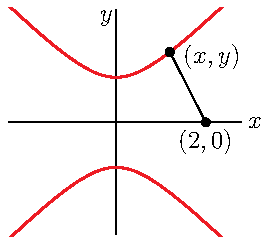
\includegraphics[scale=1]{fig/hyperbolaMaxMin.pdf}
  %\end{center}
\end{ex}

\begin{sol}
  \begin{itemize}\setlength\itemsep{0em}
    \item[]
    \item 最小化距離平方 $\equiv$ 最小化距離. 
    \item 令 $\ell$ 為 $(2, 0)$ 至 $y^2 = x^2 + 1$ 之距離: $\ds\ell^2 = (x - 2)^2 + y^2 = (x - 2)^2 + (x^2 + 1)$. 
    \item 由 $\ds\ell^2(\pm\infty)=\infty$, $\ds\ell^2(0) = 5 < \infty$, $\ell^2$ 在 $(-\infty, \infty)$ 有最小值. 
    \item 
      \begin{itemize}\setlength\itemsep{0em}
        \item $\ds\diff{}{x} \ell^2(x) = 2(x - 2) + 2x = 4(x - 1)$, 臨界點為 $1$; $\ell^2(1) = (1 - 2)^2 + (1 + 1) = 3\ie \ell(1) = \sqrt{3}$. 
        \item $\ell^2$ 在 $(-\infty,\,\infty)$ 可微, 無奇異點. 
        \item $(-\infty,\,\infty)$ 無邊界點. 
      \end{itemize}
      故最短距離為 $\ell(1) = \sqrt{3}$. 
    \end{itemize}
\end{sol}

%\begin{ex}
%  求總表面積為 $A$ 之圓柱體之最大體積.
%\end{ex}
%
%\begin{sol}
%  令圓柱體底面圓半徑為 $r$, 圓柱體高為 $h$. 由 $\ds A = 2 \pi r^2 + h\cdot 2\pi r$ $\ie$ $\ds h = \frac{A - 2\pi r^2}{2\pi r}$. 則圓柱體體積 $V(r)$ 為 $\ds V(r) = \pi r^2 \cdot h = \pi r^2\cdot\frac{A - 2\pi r^2}{2\pi r} = \frac{A}{2}r - \pi r^3$. 求臨界點 $r^\star$ 使 $V'(r^\star) = 0$ $\ie$ $\ds\frac{A}{2} - 3\pi(r^\star)^2 = 0$ $\ie$ $\ds r^\star = \sqrt{\frac{A}{6\pi}}$. 故最大體積為 $\ds\frac{A}{2}\sqrt{\frac{A}{6\pi}} - \pi\bigg(\sqrt{\frac{A}{6\pi}}\bigg)^3 = \frac{A^{\frac{3}{2}}}{3\sqrt{6\pi}}$.
%\end{sol}

\begin{ex}
  Fermat 原理: 光的行進走需時最短路徑. 如下圖, 試由 Fermat 原理推導 Snell 法則: $\ds\frac{\sin\theta_i}{\sin\theta_r} = \frac{c_a}{c_w}$, 其中 $c_a$, $c_w$ 分別為光在空氣與在水中之速度. 
  \begin{center}
    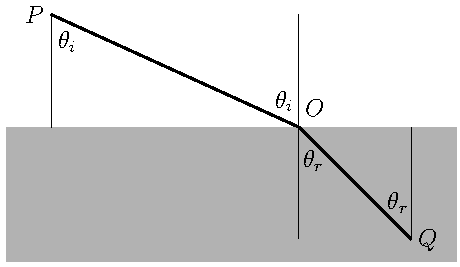
\includegraphics[scale=0.95,page=1]{fig/snell.pdf}
    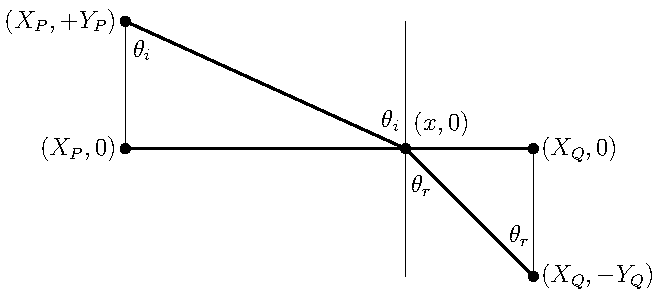
\includegraphics[scale=0.95,page=1]{fig/snellB.pdf}
  \end{center}
\end{ex}

\begin{sol}
  \begin{itemize}\setlength\itemsep{0em}
    \item[]
    \item 令光從點 $P$ 至 $Q$ 需時為 $T$, 則 $\ds T(x) = \frac{1}{c_a}\,\sqrt{(X_P-x)^2+Y_P^2} + \frac{1}{c_w}\,\sqrt{(X_Q-x)^2+Y_Q^2}\;$ $\ds\Big(\text{時間}\equiv\frac{\text{距離}}{\text{速度}}\Big)$ 
    \item $\ds T(\pm\infty) = \infty$, $\ds T(0) = \frac{1}{c_a}\,\sqrt{X_P^2+Y_P^2} + \frac{1}{c_w}\,\sqrt{X_Q^2+Y_Q^2} < \infty$, 故 $T$ 在 $(-\infty,\,\infty)$ 有最小值. 
    \item $T$ 在 $(-\infty,\,\infty)$ 可微, 無奇異點, $(-\infty,\,\infty)$ 無邊界點; $T$ 在 $(-\infty,\,\infty)$ 之最小值出現於臨界點.  
    \item 解 $\ds T'(x^\star) = 0$; 在臨界點 $\ds x^\star$ 時
      \begin{align*}
        0 &= \frac{1}{c_a}\,\frac{X_P-x^\star}{\sqrt{(X_P-x^\star)^2+Y_P^2}} + \frac{1}{c_w}\,\frac{X_Q-x^\star}{\sqrt{(X_Q-x^\star)^2+Y_Q^2}} = \frac{-\sin\theta_i}{c_a} + \frac{\sin\theta_r}{c_w}\ie\frac{\sin\theta_i}{\sin\theta_r} = \frac{c_a}{c_w}
      \end{align*}
  \end{itemize}
\end{sol}

\begin{ex}
  如圖, 若桿子可在 $3$m 寬水平走廊移動, 且無彎折通過 $2$m 寬垂直走廊, 求最大桿長. 
  \begin{center}
    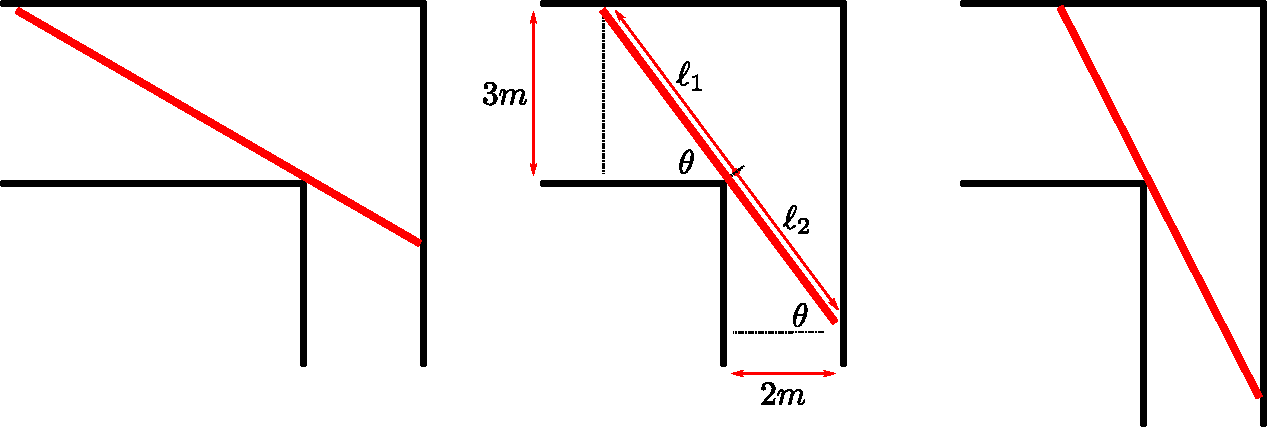
\includegraphics[height=4.2cm]{fig/corridor.pdf}
  \end{center}
\end{ex}

\begin{sol}
  \begin{itemize}\setlength\itemsep{0em}
    \item[]
    \item 如圖, 令桿與 $3$m 寬走廊內沿夾角為 $\theta$, 則總桿長為 $\ds \ell(\theta) = \ell_1(\theta) +\ell_2(\theta) = \frac{3}{\sin\theta}+\frac{2}{\cos\theta},\;0 < \theta < \frac{\pi}{2}$. 
    \item $\ds\ell(\theta)$ 最小值 $\equiv$ 最大桿長 
    \item $\ds\lim_{\theta\to 0+}\ell(\theta) = \infty$, $\ds\lim_{\theta\to\frac{\pi}{2}-}\ell(\theta) = \infty$, $\ds\ell\big(\frac{\pi}{4}\big) = \frac{5}{\sqrt{2}} < \infty$, 故 $\ell(\theta)$ 在 $\ds\big(0,\,\frac{\pi}{2}\big)$ 有最小值. 
    \item $\ds\big(0,\,\frac{\pi}{2}\big)$ 無邊界點, $\ds\ell(\theta)$ 在 $\ds\big(0,\,\frac{\pi}{2}\big)$ 可微, 無奇異點. 
    \item 求臨界點, 亦即 $\ds\ell'(\theta) = 0$ 之根 $\theta^\star$: $\ds\ell'(\theta) = -\frac{3 \cos\theta}{\sin^2\theta} + \frac{2\sin\theta}{\cos^2\theta} = \frac{-3\cos^3\theta +2 \sin^3\theta}{\sin^2\theta\cos^2\theta} = 0\ie\tan\theta^\star = \sqrt[3]{\frac{3}{2}}$. 則最大桿長為 $\ds\ell(\theta^\star) = \frac{3}{\sin\theta^\star} + \frac{2}{\cos\theta^\star} =\frac{3}{\frac{\root 3\of 3}{\sqrt{2^{\frac{2}{3}}+3^{\frac{2}{3}}}}} +\frac{2}{\frac{\root 3\of 2}{\sqrt{2^{\frac{2}{3}}+3^{\frac{2}{3}}}}} = {\big(2^{\frac{2}{3}}+3^{\frac{2}{3}}\big)}^{\frac{3}{2}}\;(\approx 7.02 \text{m})$
  \end{itemize}
\end{sol}

\section*{3.4 作圖}

\vspace{1em}

\begin{center}
  \begin{multicols}{4}
    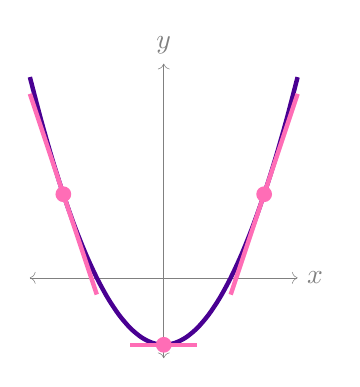
\begin{tikzpicture}[scale=0.85]
      \myaxis{x}{2}{2}{y}{1.2}{3.2}
      \draw[ultra thick, C1] plot[domain=-2:2,smooth](\x,{(\x*\x-1)});
      \draw[ultra thick, M4] plot[domain=-2:-1,smooth](\x,{1.25-4.5-3*\x});
      \draw (-1.5,1.25) node[M4, vertex]{};
      \draw[ultra thick, M4] plot[domain=-.5:.5,smooth](\x,{-1});
      \draw (0,-1) node[M4, vertex]{};
      \draw[ultra thick, M4] plot[domain=1:2,smooth](\x, {1.25-4.5+3*\x});
      \draw (1.5,1.25) node[M4, vertex]{};
    \end{tikzpicture}
    \columnbreak
    \begin{itemize}%\setlength\itemsep{0em}
      \item 切線斜率遞增 
      \item $f''(x)>0$
      \item 凹向上 
      \item 切線在圖形下方
    \end{itemize}
    \columnbreak
    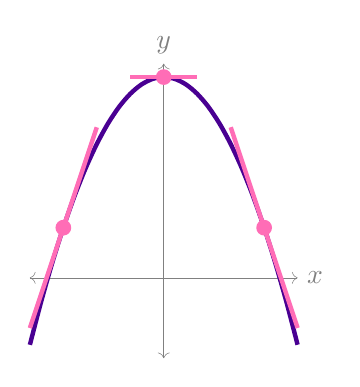
\begin{tikzpicture}[scale=0.85]
      \myaxis{x}{2}{2}{y}{1.2}{3.2}
      \draw[ultra thick, C1] plot[domain=-2:2,smooth](\x,{(-\x*\x+3)});
      \draw[ultra thick, M4] plot[domain=-2:-1,smooth](\x,{3/4+3*(\x+1.5)});
      \draw (-1.5,3/4) node[M4, vertex]{};
      \draw[ultra thick, M4] plot[domain=-.5:.5,smooth](\x,{3});
      \draw (0,3) node[M4, vertex]{};
      \draw[ultra thick, M4] plot[domain=1:2,smooth](\x, {3/4-3*(\x-1.5)});
      \draw (1.5,3/4) node[M4, vertex]{};
    \end{tikzpicture}
    \columnbreak
    \begin{itemize}%\setlength\itemsep{0em}
      \item 切線斜率遞減 
      \item $f''(x)<0$
      \item 凹向下
      \item 切線在圖形上方
    \end{itemize}
  \end{multicols}
\end{center}

\vspace{1em}

\begin{dfn}[反曲點 (inflection point) ]
  $x_0$ 為 $y = f(x)$ 的反曲點, 若
  \begin{multicols}{2}
    \begin{itemize}\setlength\itemsep{0em}
      \item $y = f(x)$ 在 $x = x_0$ 有切線. 
      \item $f$ 的凹向在 $x_0$ 的左右兩邊恰相反. 
    \end{itemize}
  \end{multicols}
\end{dfn}

\begin{prp}
  令 $f:I\to\mathbb{R}$ 為可微. 
  \begin{itemize}\setlength\itemsep{0em}
    \item 若 $f'$ 在 $I$ 嚴格遞增 ($f'' > 0$ 在 $I$) , $f$ 在 $I$ 凹向上 (上凹) . 
    \item 若 $f'$ 在 $I$ 嚴格遞減 ($f'' < 0$ 在 $I$) , $f$ 在 $I$ 凹向下 (下凹) . 
    \item 若 $f''(x_0) = 0$, 則 $x_0\in I$ 為 $f$ 的反曲點.  
  \end{itemize}
\end{prp}

\vspace{1em}

\begin{center}
  \begin{tikzpicture}[yscale=0.6]
    \draw[ultra thick, C1] plot[domain=-2.12:.5,smooth](\x,{\x*\x});
    \draw[ultra thick, C1] plot[domain=.5:6.28,smooth](\x-.02,{sin(\x r)-.25});
    \draw[ultra thick, C1] plot[domain=6.28:8,smooth](\x,{(\x-5.75)*(\x-5.78)-.5});
    \draw[thick, M4, <->] (-2.12,-2.5)--(0.5,-2.5); \draw[M4] (-.75,-3) node{凹向上};
    \draw[dashed, M4, pattern=north east lines, pattern color=M4] (-2.12,-2.5)--(-2.12,4.5)--(.5,4.5)--(.5,-2.5);
    \draw[thick, M3, <->] (.5,-2.5)--(3.16,-2.5); \draw[M3] (1.75,-3) node{凹向下};
    \draw[dashed, M3, pattern=north west lines, pattern color=M3] (3.16,-2.5)--(3.16,4.5)--(.5,4.5)--(.5,-2.5);
    \draw[thick, M4, <->] (3.16,-2.5)--(8,-2.5); \draw[M4] (5,-3) node{凹向上};
    \draw[dashed, M4, pattern=north east lines, pattern color=M4] (3.16,-2.5)--(3.16,4.5)--(8,4.5)--(8,-2.5);
    \draw (.5,.25) node[vertex](a){}; \draw (3.16,-.25) node[vertex](b){};
    \draw[<-] (a)--(.5,-.75) node[below]{反曲點};
    \draw[<-] (b)--(3.17,.75) node[above]{反曲點};
    \draw (.5,-1.4) node[below]{$f''(x)$ 變號};
  \end{tikzpicture}
\end{center}

\begin{center}
  
\begin{tikzpicture}[scale=0.4]
    \draw[M4, ultra thick] (-1.2, 0.7) -- (-0.2, 0.7);
    \draw[M4, ultra thick] (-0.7, 0.2) -- (-0.7, 1.2);
    \draw[M4, ultra thick] (1.2, 0.7) -- (0.2, 0.7);
    \draw[M4, ultra thick] (0.7, 0.2) -- (0.7, 1.2);
    \draw[M4, ultra thick] (-1, 0) arc [start angle = -180, end angle = 0, radius = 1] (1, 0);
  \end{tikzpicture}
  \hspace{1cm}
  
\begin{tikzpicture}[scale=0.4]
    \draw[M4, ultra thick] (-1.2, 0.7) -- (-0.2, 0.7);
    \draw[M4, ultra thick] (1.2, 0.7) -- (0.2, 0.7);
    \draw[M4, ultra thick] (1, -1) arc [start angle = 0, end angle = 180, radius = 1] (-1, -1);
  \end{tikzpicture}
\end{center}

\begin{center}
  \begin{tabular}{ccc}
    \toprule
    & 嚴格遞減 ($-$) & 嚴格遞增 ($+$)  \\
    \midrule
    凹向上 ($+$) & 
    \parbox{3cm}{
        \begin{tikzpicture}[scale=1]
        \myaxis{x}{1.2}{1.2}{y}{1.2}{1.2}
        \draw[thick, C4] plot[domain=-0.98:0.98,smooth] (\x, {1 + 0.18 - sqrt(4 - (\x - 1)^2)});
      \end{tikzpicture}} & 
      \parbox{3cm}{\begin{tikzpicture}[scale=1]
        \myaxis{x}{1.2}{1.2}{y}{1.2}{1.2}
        \draw[thick, C4] plot[domain=-0.98:0.98,smooth] (\x, {1 + 0.18 - sqrt(4 - (\x + 1)^2)});
      \end{tikzpicture}} \\
    \midrule
    凹向下 ($-$) & 
    \parbox{3cm}{
        \begin{tikzpicture}[scale=1]
        \myaxis{x}{1.2}{1.2}{y}{1.2}{1.2}
        \draw[thick, C4] plot[domain=-0.98:0.98,smooth] (\x, {-1 - 0.18 + sqrt(4 - (\x + 1)^2)});
      \end{tikzpicture}} & 
      \parbox{3cm}{
        \begin{tikzpicture}[scale=1]
        \myaxis{x}{1.2}{1.2}{y}{1.2}{1.2}
        \draw[thick, C4] plot[domain=-0.98:0.98,smooth] (\x, {-1 - 0.18 + sqrt(4 - (\x - 1)^2)});
      \end{tikzpicture}} \\
    \bottomrule
  \end{tabular}
\end{center}

\begin{prp}[漸近線 (asymptote) ]
  \begin{itemize}\setlength\itemsep{0em}
    \item[]
    \item 若 $\ds\lim_{x\to a-}f(x) = \pm\infty$ 或 $\ds\lim_{x\to a+}f(x) = \pm\infty$, $f$ 在 $a$ 有垂直漸近線.  
    \item 若 $\ds\lim_{x\to-\infty}f(x) = L$ 或 $\ds\lim_{x\to\infty}f(x) = L$, $f$ 有水平漸近線 $\ds y = L$.  
    \item 若 $\ds\lim_{x\to-\infty}(f(x) - (m x + n)) = 0$ 或 $\ds\lim_{x\to\infty}(f(x) - (m x + n)) = 0$, $m\ne 0$, 則 $f$ 有斜漸近線 $\ds y = m x + n$: 斜漸近線 $\ds y = mx + n$ 由極限 $\ds m = \lim_{x\to\pm\infty}\frac{f(x)}{x}$ 與 $\ds n = \lim_{x\to\pm\infty}(f(x) - mx)$ 之存在性決定. 
  \end{itemize}
\end{prp}

\begin{fact}[作圖步驟]
  \begin{itemize}\setlength\itemsep{0em}
    \item[]
    \item 觀察定義域, 對稱性, 週期性. 
    \item 決定漸近線. 
    \item 解 $f'(x) = 0$, $f''(x) = 0$ 並決定 $f'$, $f''$ 之正負區間; 製表. 
    \item 依表判斷 $f$ 之升降, 凹向, 臨界點, 奇異點, 反曲點; 作圖. 
  \end{itemize}
\end{fact}

\begin{ex}
  決定 $\ds f(x) = x^4 - 2 x^3 + 1$ 的升降, 凹向, 臨界點, 奇異點, 反曲點並作圖. 
\end{ex}

\begin{sol}
  \begin{itemize}\setlength\itemsep{0em}
    \item[]
    \item $\ds f'(x) = 4 x^3 - 6 x^2 = 4 x^2\big(x - \frac{3}{2}\big)$; $\ds f''(x) = 12 x^2 - 12 x = 12x(x - 1)$. 
    \item 製表: 
      \begin{center}
        \begin{tikzpicture}[scale=2]
        \draw (0, 0)--(4, 0);
        \foreach \x/\y in {0/1, 1/2, \frac{3}{2}/3}{
        \node at (\y, -0.25) {$\x$};
        \draw[xshift=\y cm] (0, 0) -- (0, 0.45);}
        \foreach \x/\y in {0/$-$, 1/$-$, 2/$-$, 3/$+$}
        \node at (\x + 0.5, 0.25) {\y};
        \foreach \x/\y in {0/$+$, 1/$-$, 2/$+$, 3/$+$}
        \node at (\x + 0.5, -0.25) {\y};
        \node at (4, -0.25) {$f''$};
        \node at (4, 0.25) {$f'$};
        \end{tikzpicture}
      \end{center}
    \item 臨界點 ($f' = 0$) : $x = 0$ 與 $\ds x = \frac{3}{2}$
    \item 嚴格遞增區間 ($f' > 0$) : $\ds \big(\frac{3}{2}, \infty\big)$
    \item 嚴格遞減區間 ($f' < 0$) : $\ds \big(-\infty, \frac{3}{2}\big)$
    \item 反曲點 ($f'' = 0$ 且前後 $f''$ 異號處) : $x = 0$ 與 $x = 1$
    \item 作圖: \vspace{-8mm}
      \begin{center}
        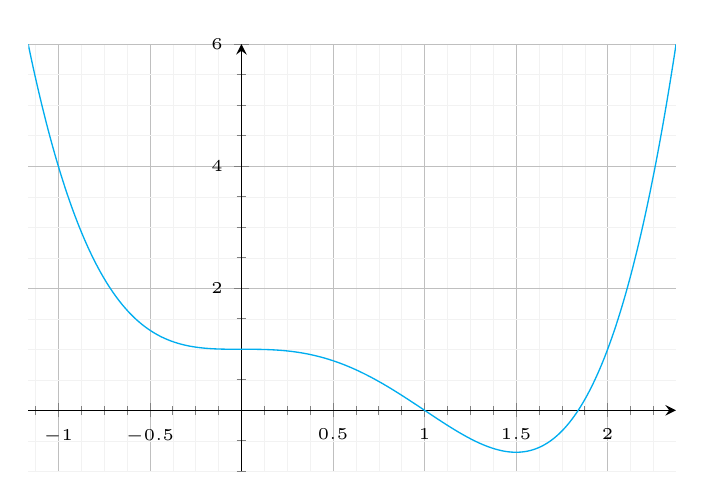
\begin{tikzpicture}[scale=1.2]
          \begin{axis}%
            [grid=both,
             unit vector ratio={3 1},
             minor tick num=3,
             ymin=-1, ymax=6,
             grid style={line width=.1pt, draw=gray!10},
             major grid style={line width=.2pt,draw=gray!50},
             axis lines=middle
            ]
            \addplot[domain=-3:3,samples=5000,smooth,cyan] {x^4 - 2* x^3 + 1};
          \end{axis}
        \end{tikzpicture}
      \end{center}
  \end{itemize}
\end{sol}

\begin{ex}
  決定 $\ds f(x) = \frac{x}{x^2 + 3}$ 之升降, 凹向, 臨界點, 奇異點, 反曲點並作圖. 
\end{ex}

\begin{sol}
  \begin{itemize}\setlength\itemsep{0em}
    \item[]
    \item $\ds f'(x) = \frac{3-x^2}{(x^2 + 3)^2} = \frac{(\sqrt{3}-x)(\sqrt{3} + x)}{(x^2 + 3)^2}$; $\ds f''(x) = \frac{2x(x+3)(x-3)}{(x^2 + 3)^3}$. 
    \item 製表: 
      \begin{center}
        \begin{tikzpicture}[scale=2]
          \draw (0, 0)--(6, 0);
          \foreach \x/\y in {-3/1, -\sqrt{3}/2, 0/3, \sqrt{3}/4, 3/5}{
          \node at (\y, -0.25) {$\x$};
          \draw[xshift=\y cm] (0, 0) -- (0, 0.45);}
          \foreach \x/\y in {0/$-$, 1/$-$, 2/$+$, 3/$+$, 4/$-$, 5/$-$}
          \node at (\x + 0.5, 0.25) {\y};
          \foreach \x/\y in {0/$-$, 1/$+$, 2/$+$, 3/$-$, 4/$-$, 5/$+$}
          \node at (\x + 0.5, -0.25) {\y};
          \node at (6, -0.25) {$f''$};
          \node at (6, 0.25) {$f'$};
        \end{tikzpicture}
      \end{center}
    \item 水平漸近線:  $y = 0$, 因 $\ds\lim_{x\to\pm\infty}\frac{x}{x^2 + 3} = 0$
    \item 嚴格遞增區間 ($f' > 0$) : $\ds (-\sqrt{3}, \sqrt{3})$
    \item 嚴格遞減區間 ($f' < 0$) : $\ds (-\infty, -\sqrt{3})$ 與 $\ds (\sqrt{3}, \infty)$
    \item 臨界點 ($f' = 0$) : $\ds x = \pm\sqrt{3}$
    \item 反曲點 ($f'' = 0$ 且前後 $f''$ 異號處) : $x = -3$ 與 $x = 0$ 與 $x = 3$
    \item 作圖: \vspace{-8mm}
      \begin{center}
        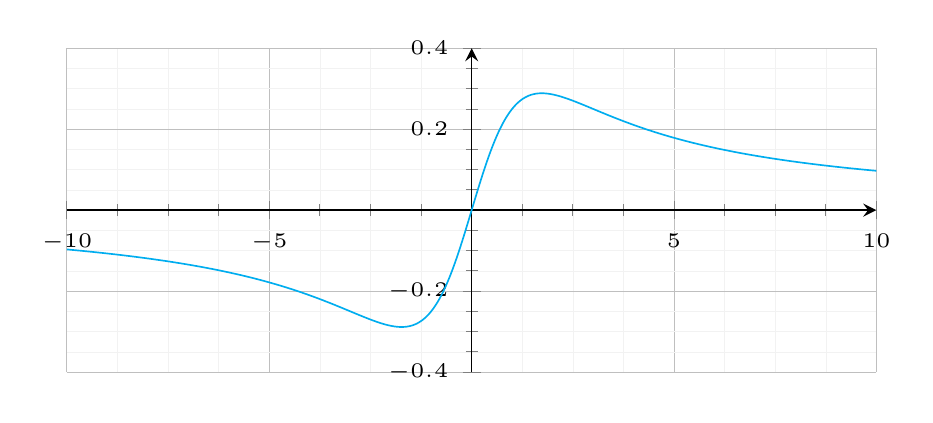
\begin{tikzpicture}[scale=1.5]
          \begin{axis}%
            [grid=both,
             unit vector ratio={1 10},
             minor tick num=3,
             ymin = -0.4, ymax = 0.4,
             grid style={line width=.1pt, draw=gray!10},
             major grid style={line width=.2pt,draw=gray!50},
             axis lines=middle
            ]
            \addplot[domain=-10:10,samples=3000,smooth,cyan] {x / (x^2 + 3)};
          \end{axis}
        \end{tikzpicture}
      \end{center}
  \end{itemize}
\end{sol}

\begin{ex}
  決定 $\ds f(x) = \frac{x^3}{x^2 - 1}$ 的升降, 凹向, 臨界點, 奇異點, 反曲點並作圖. 
\end{ex}

\begin{sol}
  \begin{itemize}\setlength\itemsep{0em}
    \item[]
    \item $\ds f'(x) = \frac{x^2(x^2 - 3)}{(x^2 -1)^2} = \frac{x^2(x - \sqrt{3})(x + \sqrt{3})}{(x^2 -1)^2}$; $\ds f''(x) = \frac{2x(x^2 + 3)}{(x^2 - 1)^3}$
    \item 製表:  
      \begin{center}
        \begin{tikzpicture}[scale=2]
          \draw (0, 0)--(6, 0);
          \foreach \x/\y in {-\sqrt{3}/1, -1/2, 0/3, 1/4, \sqrt{3}/5}{
          \node at (\y, -0.25) {$\x$};
          \draw[xshift=\y cm] (0, 0) -- (0, 0.45);}
          \foreach \x/\y in {0/$+$, 1/$-$, 2/$-$, 3/$-$, 4/$-$, 5/$+$}
          \node at (\x + 0.5, 0.25) {\y};
          \foreach \x/\y in {0/$-$, 1/$-$, 2/$+$, 3/$-$, 4/$+$, 5/$+$}
          \node at (\x + 0.5, -0.25) {\y};
          \node at (6, -0.25) {$f''$};
          \node at (6, 0.25) {$f'$};
        \end{tikzpicture}
      \end{center}
    \item 奇異點:  $\ds x^2 - 1 = 0\ie x = \pm 1$, 故垂直漸近線: $\ds x = \pm1$
    \item 斜漸近線:  $y = x$, 因 $\ds\lim_{x\to\pm\infty}\big(\frac{x^3}{x^2 - 1} - x\big) = 0$
    \item 嚴格遞增區間 ($f' > 0$) : $\ds (-\infty, -\sqrt{3})$ 與 $\ds (\sqrt{3}, \infty)$
    \item 嚴格遞減區間 ($f' < 0$) : $\ds(-\sqrt{3}, \sqrt{3})$
    \item 臨界點 ($f' = 0$) : $\ds x = 0$ 與 $\ds x = \pm\sqrt{3}$
    \item 反曲點 ($f'' = 0$ 且前後 $f''$ 異號處) : $x = 0$
    \item 作圖: \vspace{-8mm}
      \begin{center}
        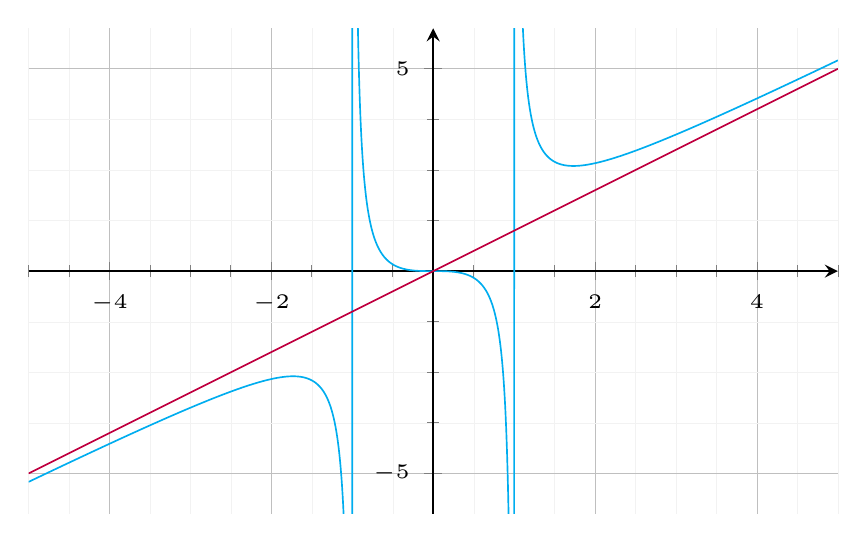
\begin{tikzpicture}[scale=1.5]
          \begin{axis}%
            [grid=both,
             unit vector ratio={2 1},
             minor tick num=3,
             ymax=6, ymin=-6,
             grid style={line width=.1pt, draw=gray!10},
             major grid style={line width=.2pt,draw=gray!50},
             axis lines=middle
            ]
            \addplot[domain=-5:5,samples=5000,smooth,cyan] {x^3 / (x^2 - 1)};
            \addplot[domain=-5:5,samples=5000,smooth,purple] {x};
          \end{axis}
        \end{tikzpicture}
      \end{center}
  \end{itemize}
\end{sol}

\end{document}
